\begingroup
\let\figure\RSIappendixfigure
\let\endfigure\RSIendappendixfigure
\subsubsection{Original four-round Llama figures}
\label{app:llama-raw-figures}

Figures~\ref{fig:llama-raw-unaudited}--\ref{fig:llama-raw-comparison-difficulty}
show the original Llama-3.2-3B-Instruct plots for rounds 0--4.
The unaudited and adaptive-audit runs are shown separately and together,
with aggregate and difficulty-stratified curves in the same grouping as
Appendix~\ref{app:qwen-raw-figures}. These are complementary views of the
same checkpoints, not additional experiments. Each uses the same 2,000 ID
or 1,000 OOD questions across checkpoints and five paired blocks.
Error bars are pointwise, descriptive 95\% block-$t$ intervals;
round zero is one shared base checkpoint, not five independent fits.

\begin{figure}[H]
\centering
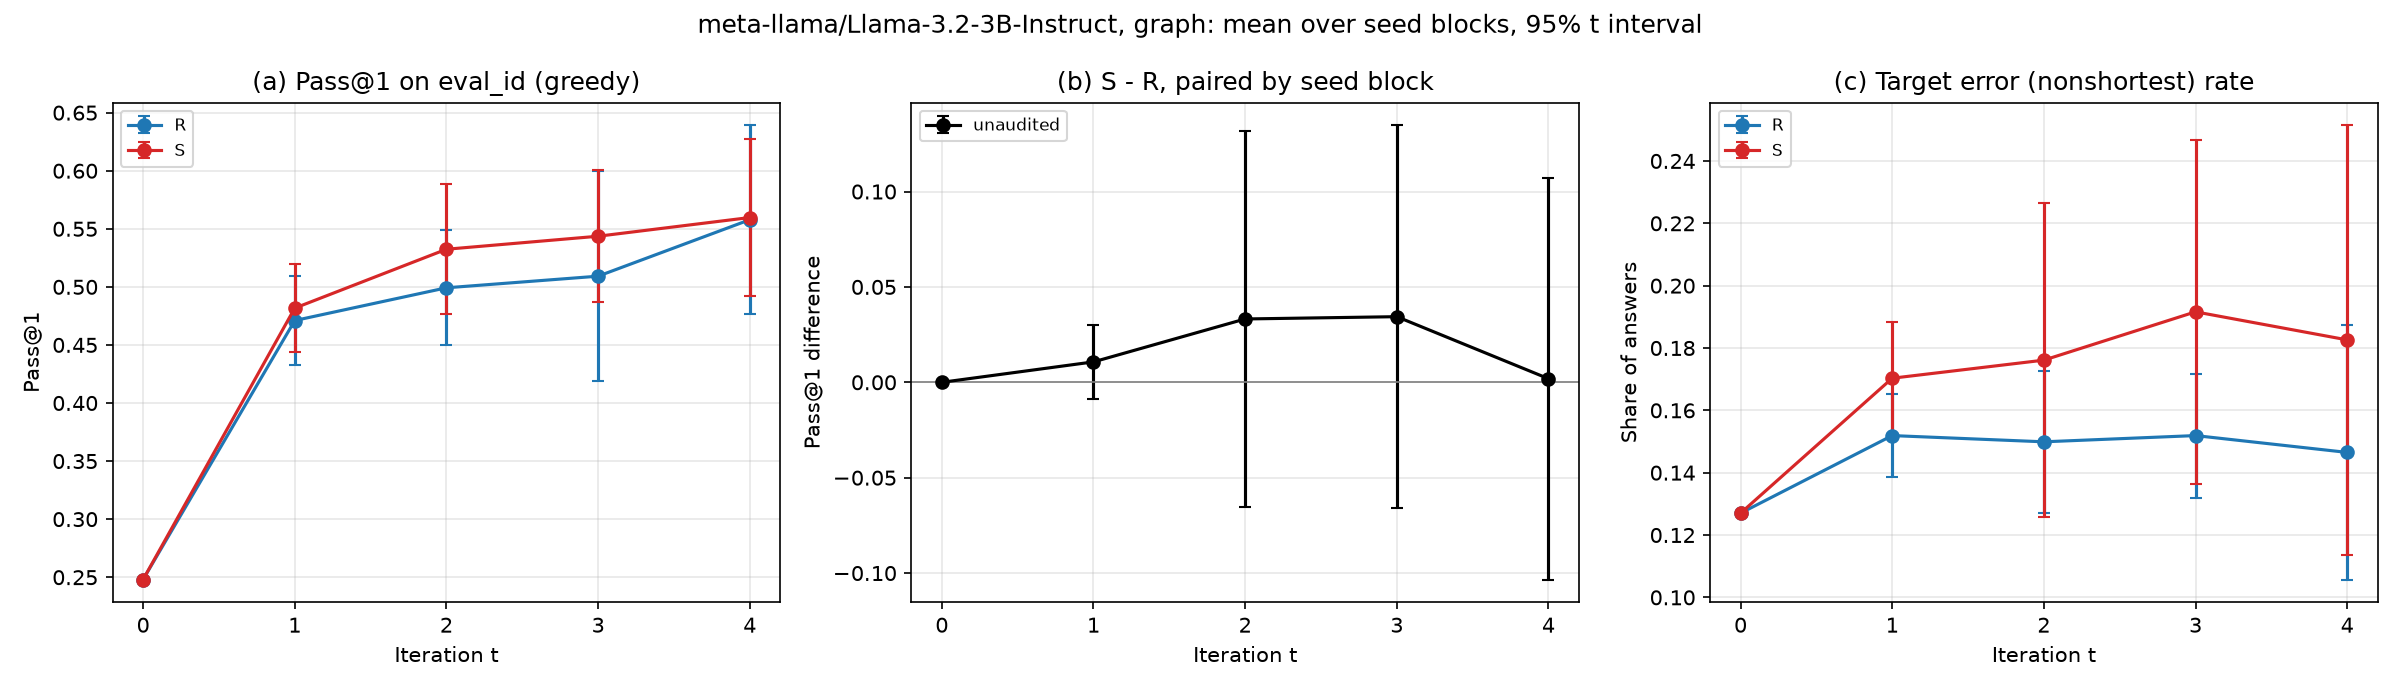
\includegraphics[width=0.90\linewidth]{figures/llama_four_round_raw/unaudited_eval_id_pass1.png}
\par\smallskip
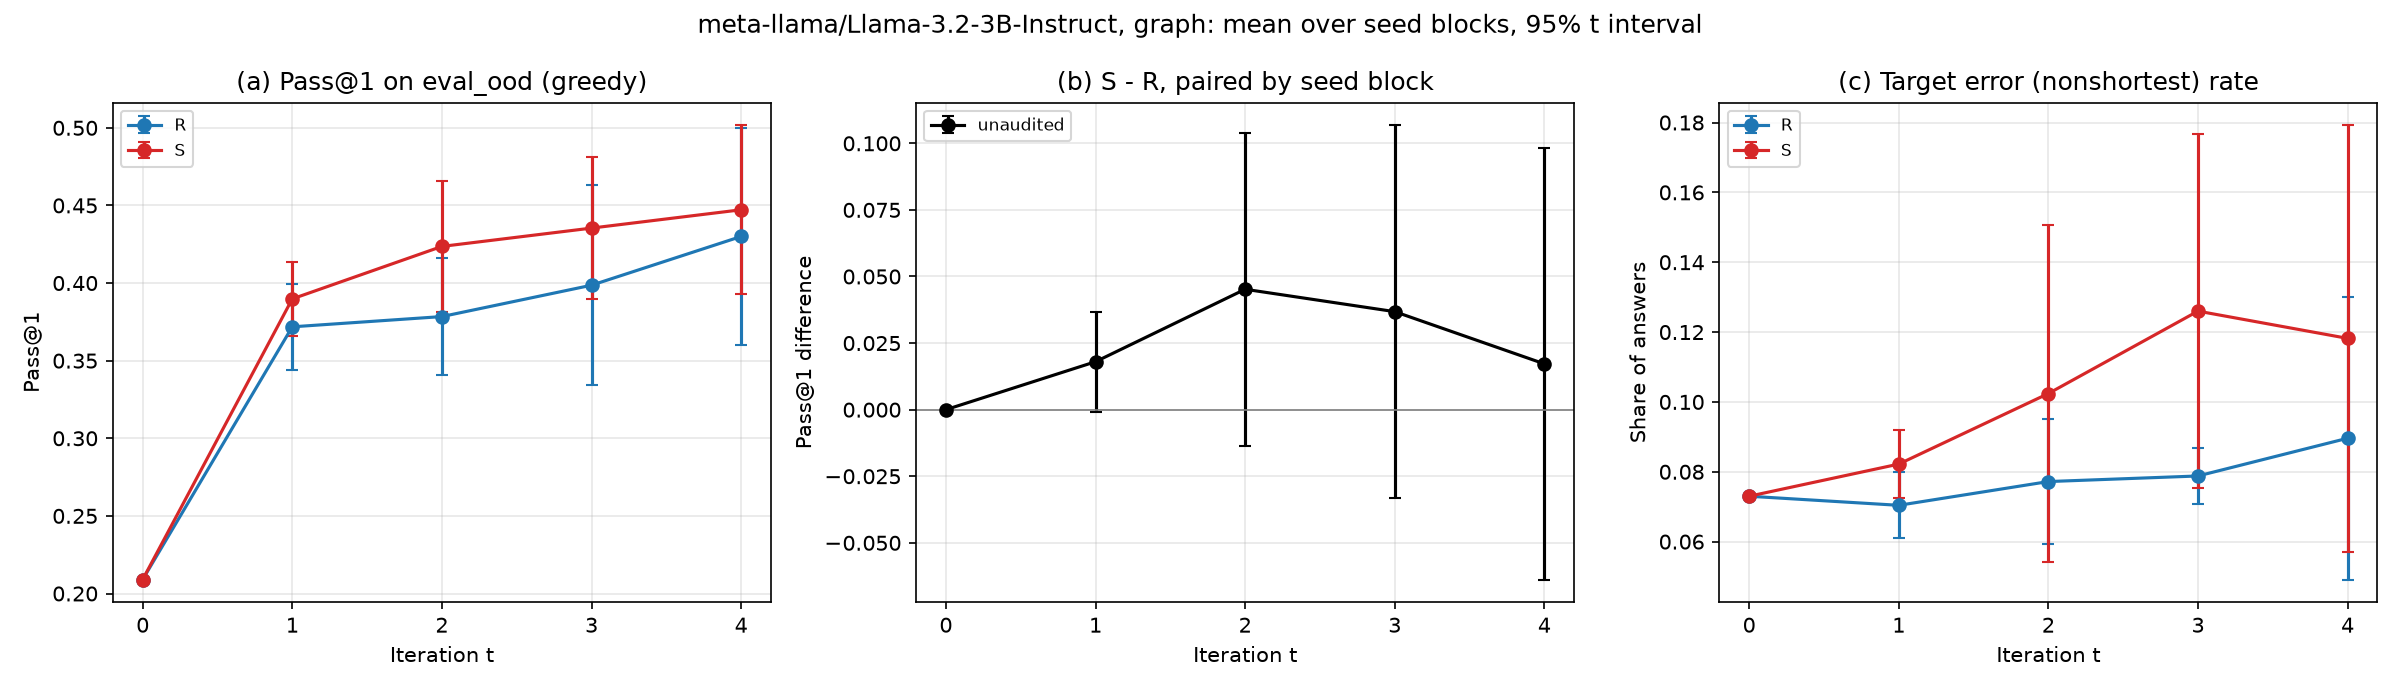
\includegraphics[width=0.90\linewidth]{figures/llama_four_round_raw/unaudited_eval_ood_pass1.png}
\caption{Original unaudited Llama-3.2-3B graph curves, ID (top) and OOD
(bottom), for rounds 0--4. The three panels show greedy Pass@1, paired
$S-R$ accuracy, and nonshortest-error incidence among all answers.}
\label{fig:llama-raw-unaudited}
\end{figure}

Both unaudited arms improve from the shared bases $0.248$ ID and
$0.209$ OOD. Round-four $R/S$ accuracy is $0.558/0.560$ ID and
$0.430/0.447$ OOD, with paired contrasts $0.002\pm0.105$ and
$0.017\pm0.081$.

\begin{figure}[H]
\centering
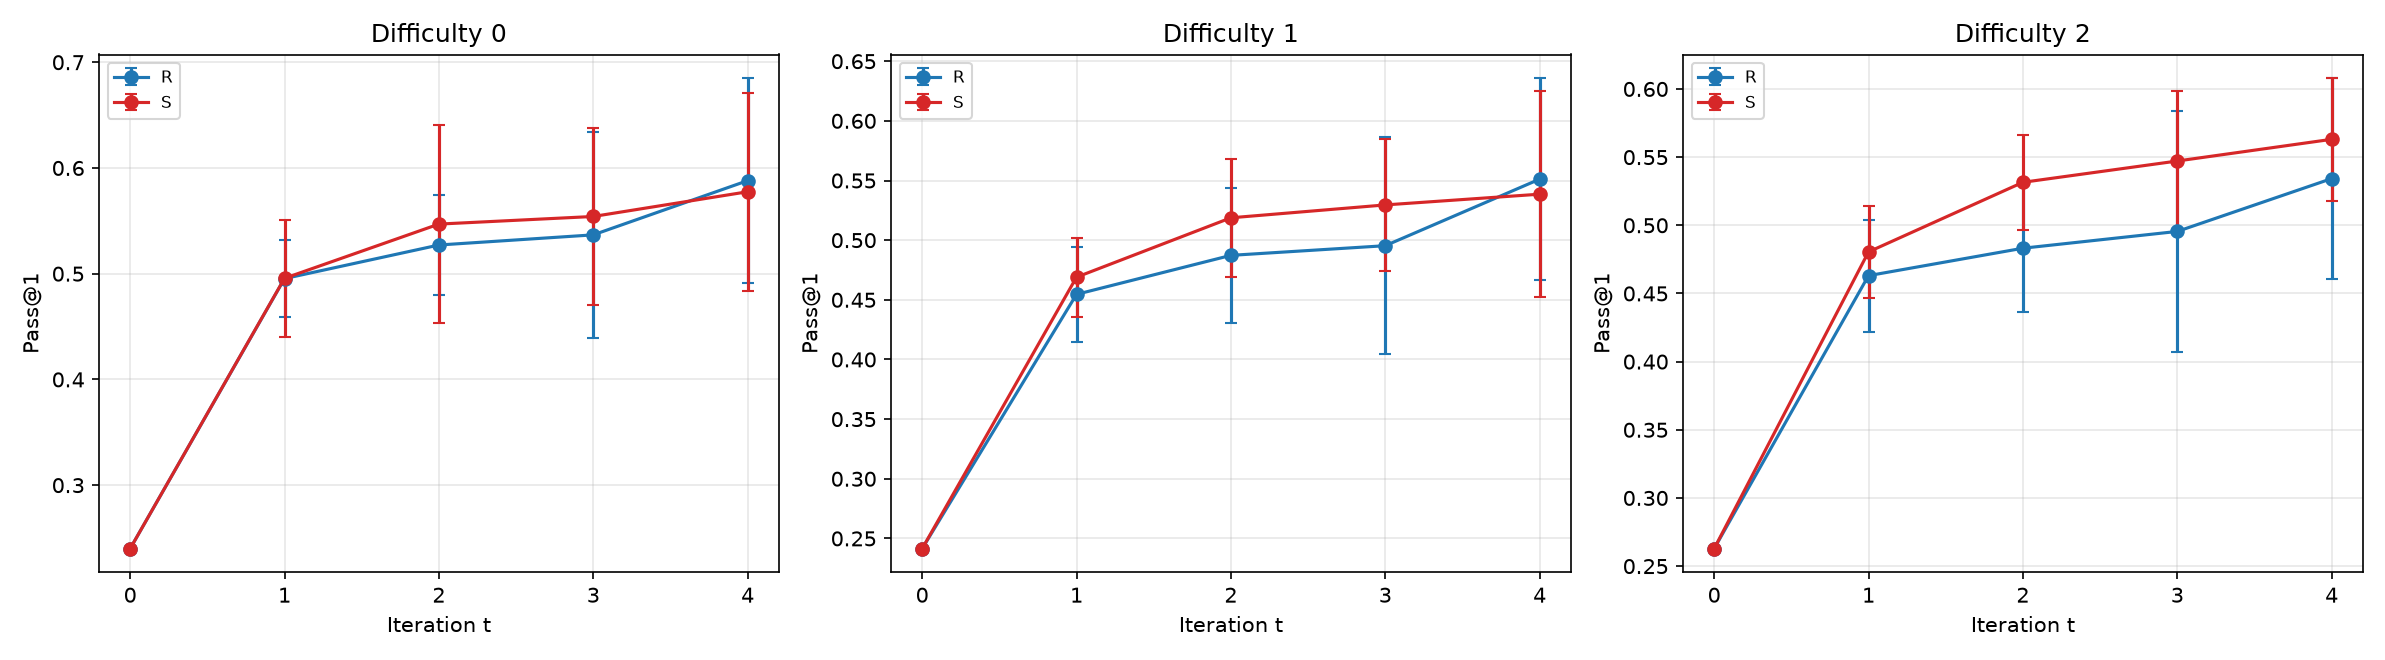
\includegraphics[width=0.90\linewidth]{figures/llama_four_round_raw/unaudited_eval_id_by_difficulty.png}
\par\smallskip
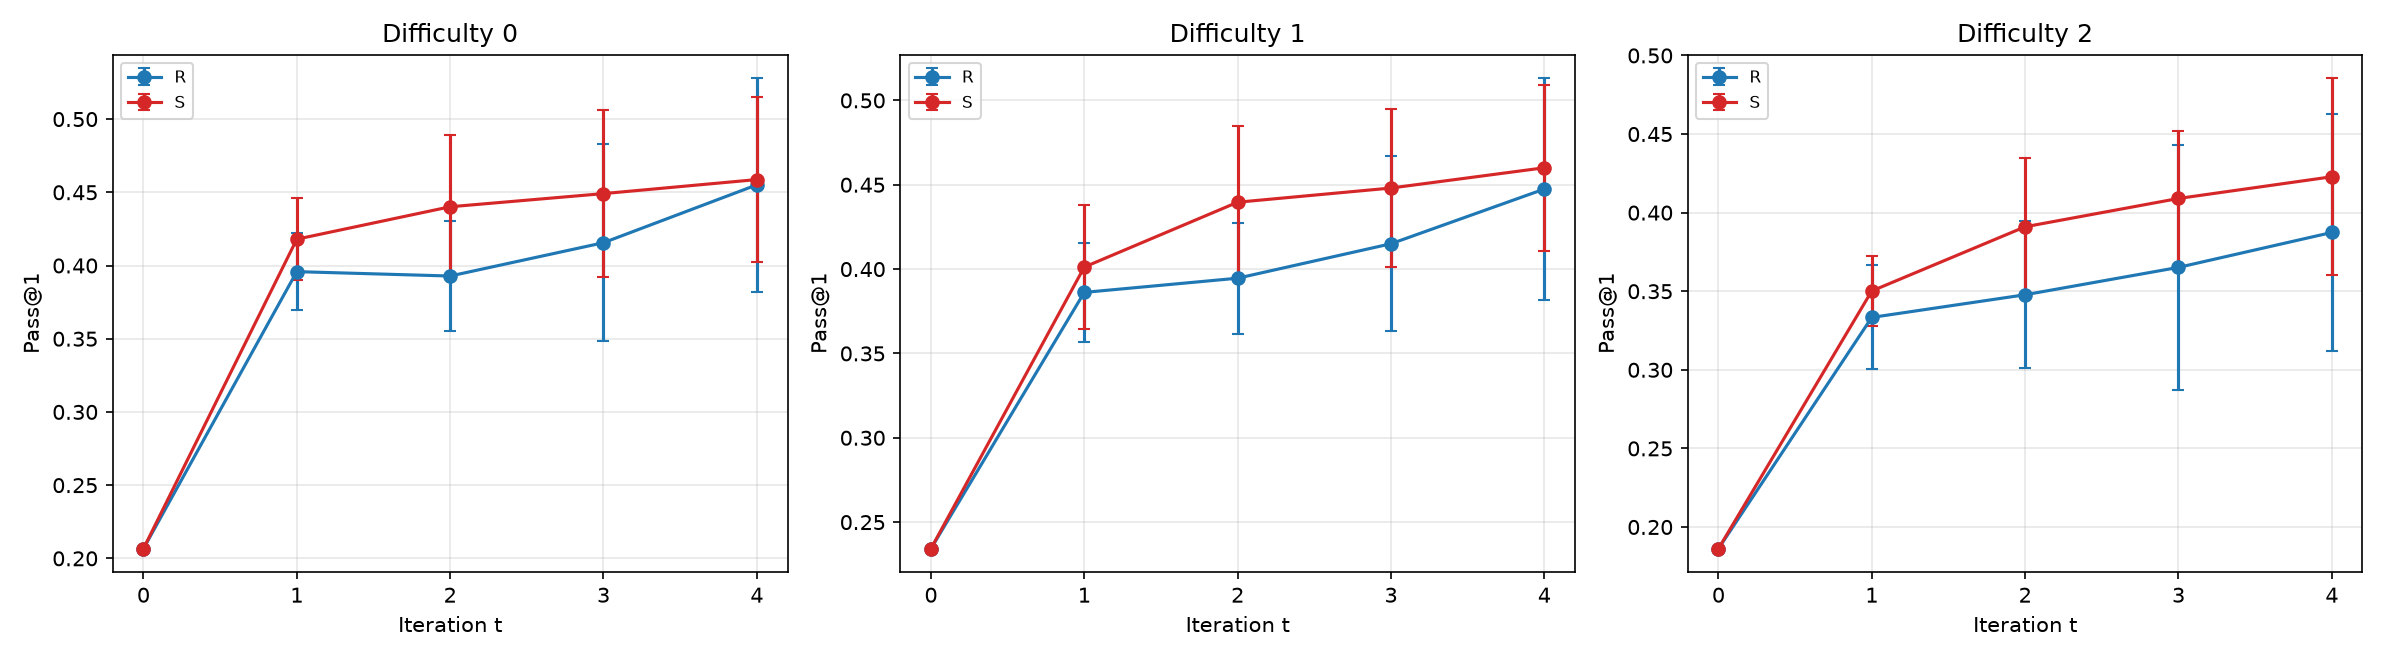
\includegraphics[width=0.90\linewidth]{figures/llama_four_round_raw/unaudited_eval_ood_by_difficulty.png}
\caption{Original unaudited Llama-3.2-3B graph accuracy by generator
difficulty stratum, ID (top) and OOD (bottom), for rounds 0--4.
Strata 0--2 run from left to right and contain $667/667/666$ ID
and $334/333/333$ OOD questions. Error bars use five paired blocks.}
\label{fig:llama-raw-unaudited-difficulty}
\end{figure}

These are fixed generator strata, not an established model-difficulty
ordering. The panel-specific vertical scales are retained, and differences
in the appearance of the curves do not constitute additional
difficulty-specific significance evidence.

\begin{figure}[H]
\centering
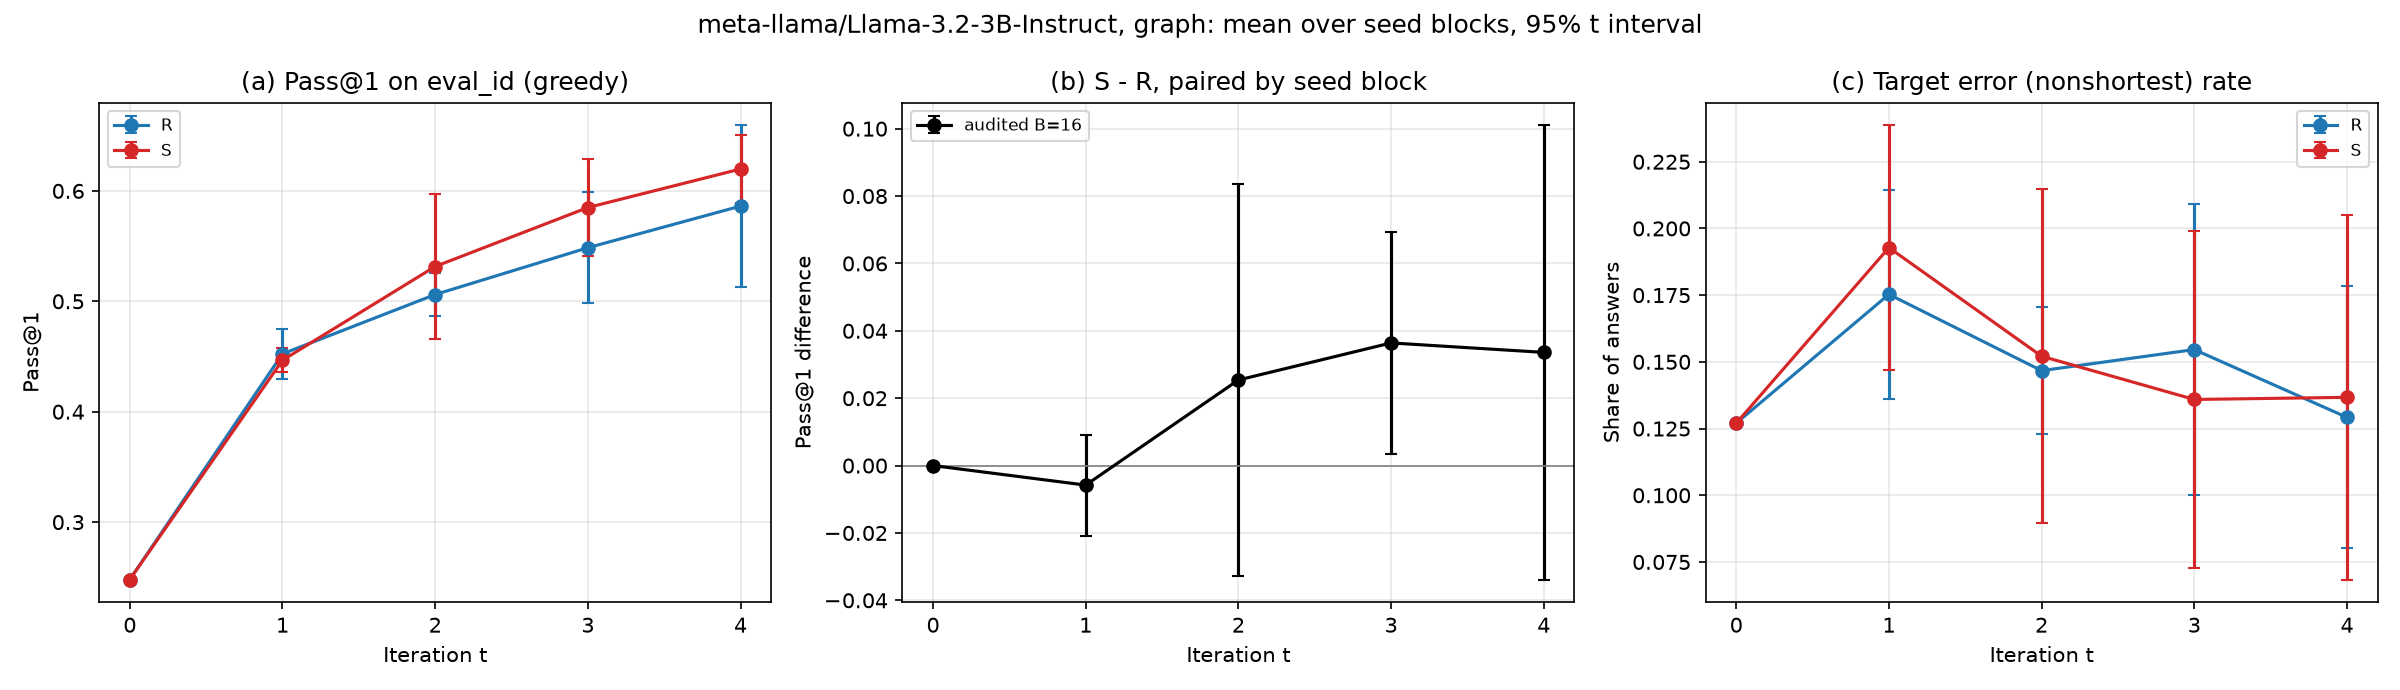
\includegraphics[width=0.90\linewidth]{figures/llama_four_round_raw/audited_eval_id_pass1.png}
\par\smallskip
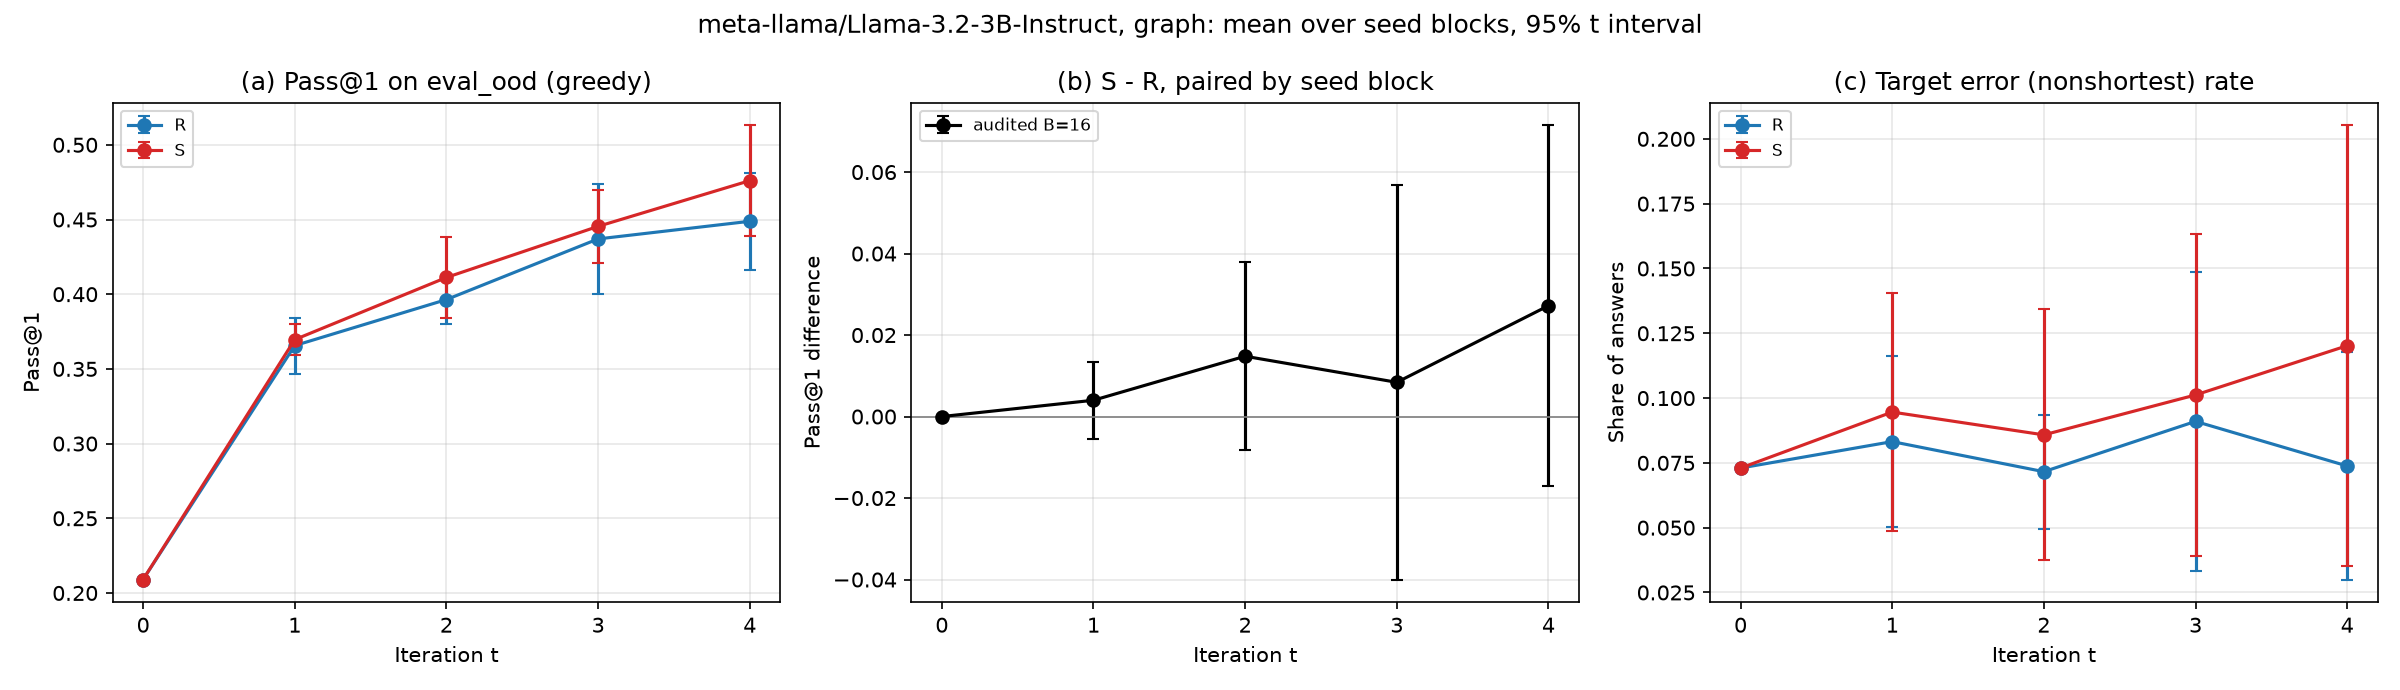
\includegraphics[width=0.90\linewidth]{figures/llama_four_round_raw/audited_eval_ood_pass1.png}
\caption{Original adaptive-audit Llama-3.2-3B graph curves, ID (top)
and OOD (bottom), with $B_{\rm qry}=16$ correctness queries per
arm-round. The panels show greedy Pass@1, paired $S-R$ accuracy,
and nonshortest-error incidence. Each audited arm spends 64 queries.}
\label{fig:llama-raw-audited}
\end{figure}

Audited round-four $R/S$ accuracy reaches $0.586/0.620$ ID and
$0.449/0.476$ OOD. The paired accuracy contrasts are
$0.034\pm0.067$ and $0.027\pm0.044$, respectively.
These are within-policy arm contrasts, not effects of auditing.

\begin{figure}[H]
\centering
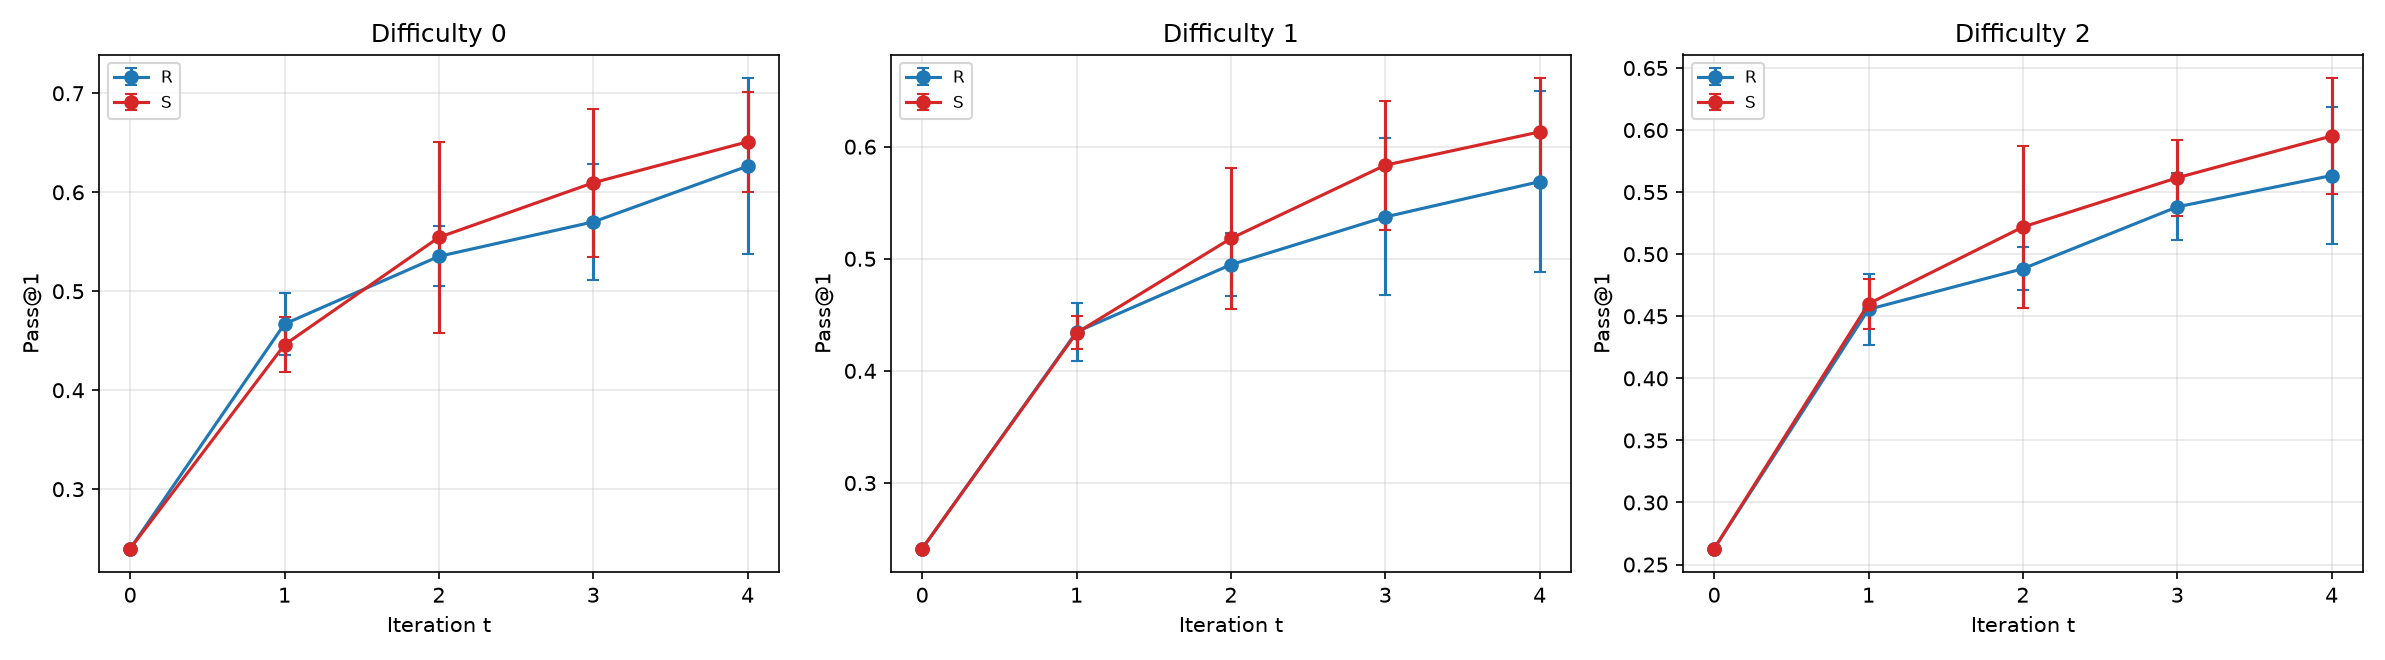
\includegraphics[width=0.90\linewidth]{figures/llama_four_round_raw/audited_eval_id_by_difficulty.png}
\par\smallskip
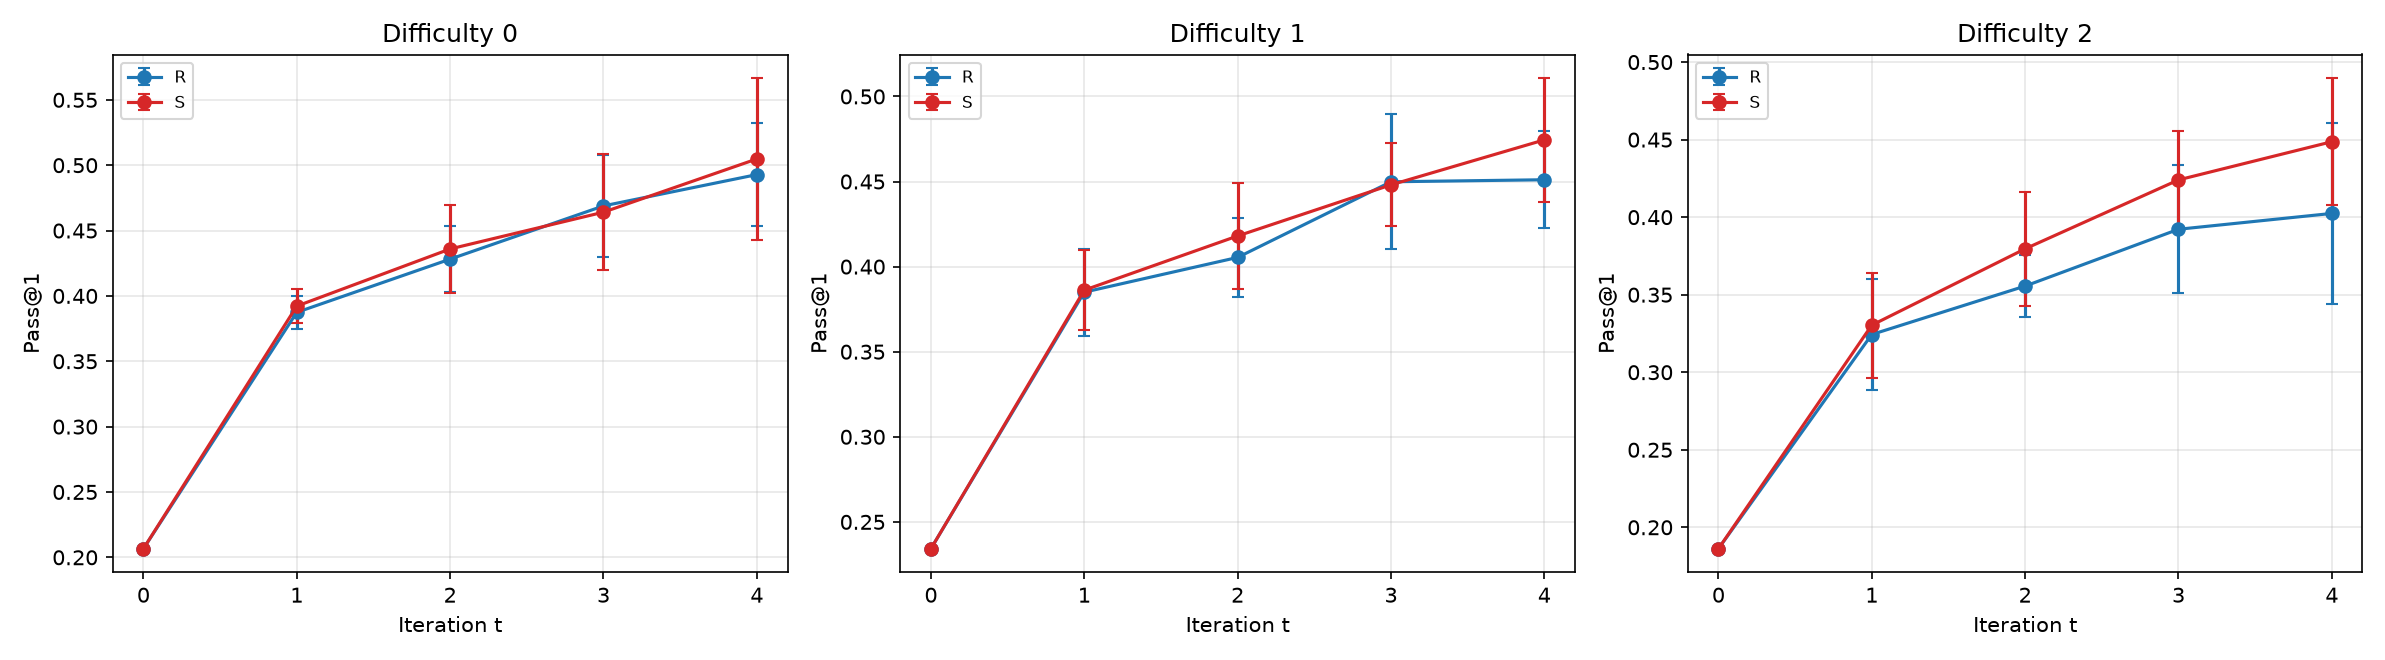
\includegraphics[width=0.90\linewidth]{figures/llama_four_round_raw/audited_eval_ood_by_difficulty.png}
\caption{Original adaptive-audit Llama-3.2-3B graph accuracy by
generator stratum, ID (top) and OOD (bottom), for rounds 0--4.
The fixed question strata and pointwise block-$t$ intervals follow
Figure~\ref{fig:llama-raw-unaudited-difficulty}.}
\label{fig:llama-raw-audited-difficulty}
\end{figure}

The audited curves show heterogeneous trajectories across the generator
strata. They retain separate vertical scales and use the same question
sets as the unaudited curves. This descriptive breakdown does not
establish stratum-specific audit benefits.

\begin{figure}[H]
\centering
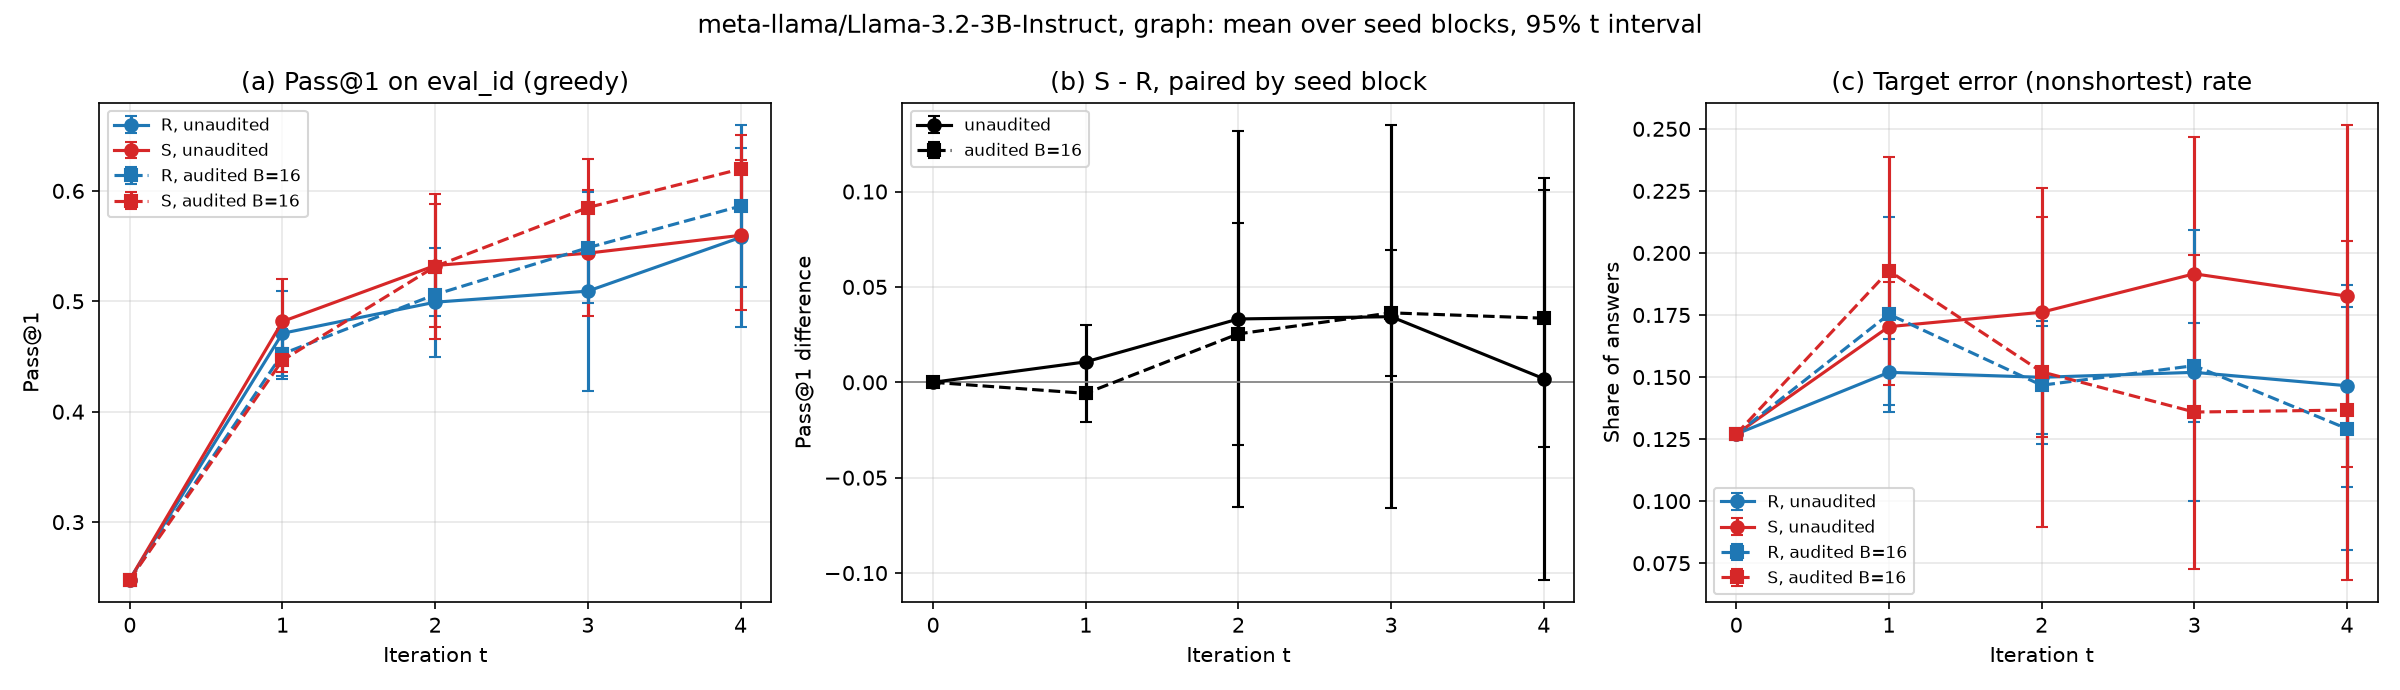
\includegraphics[width=0.90\linewidth]{figures/llama_four_round_raw/comparison_eval_id_pass1.png}
\par\smallskip
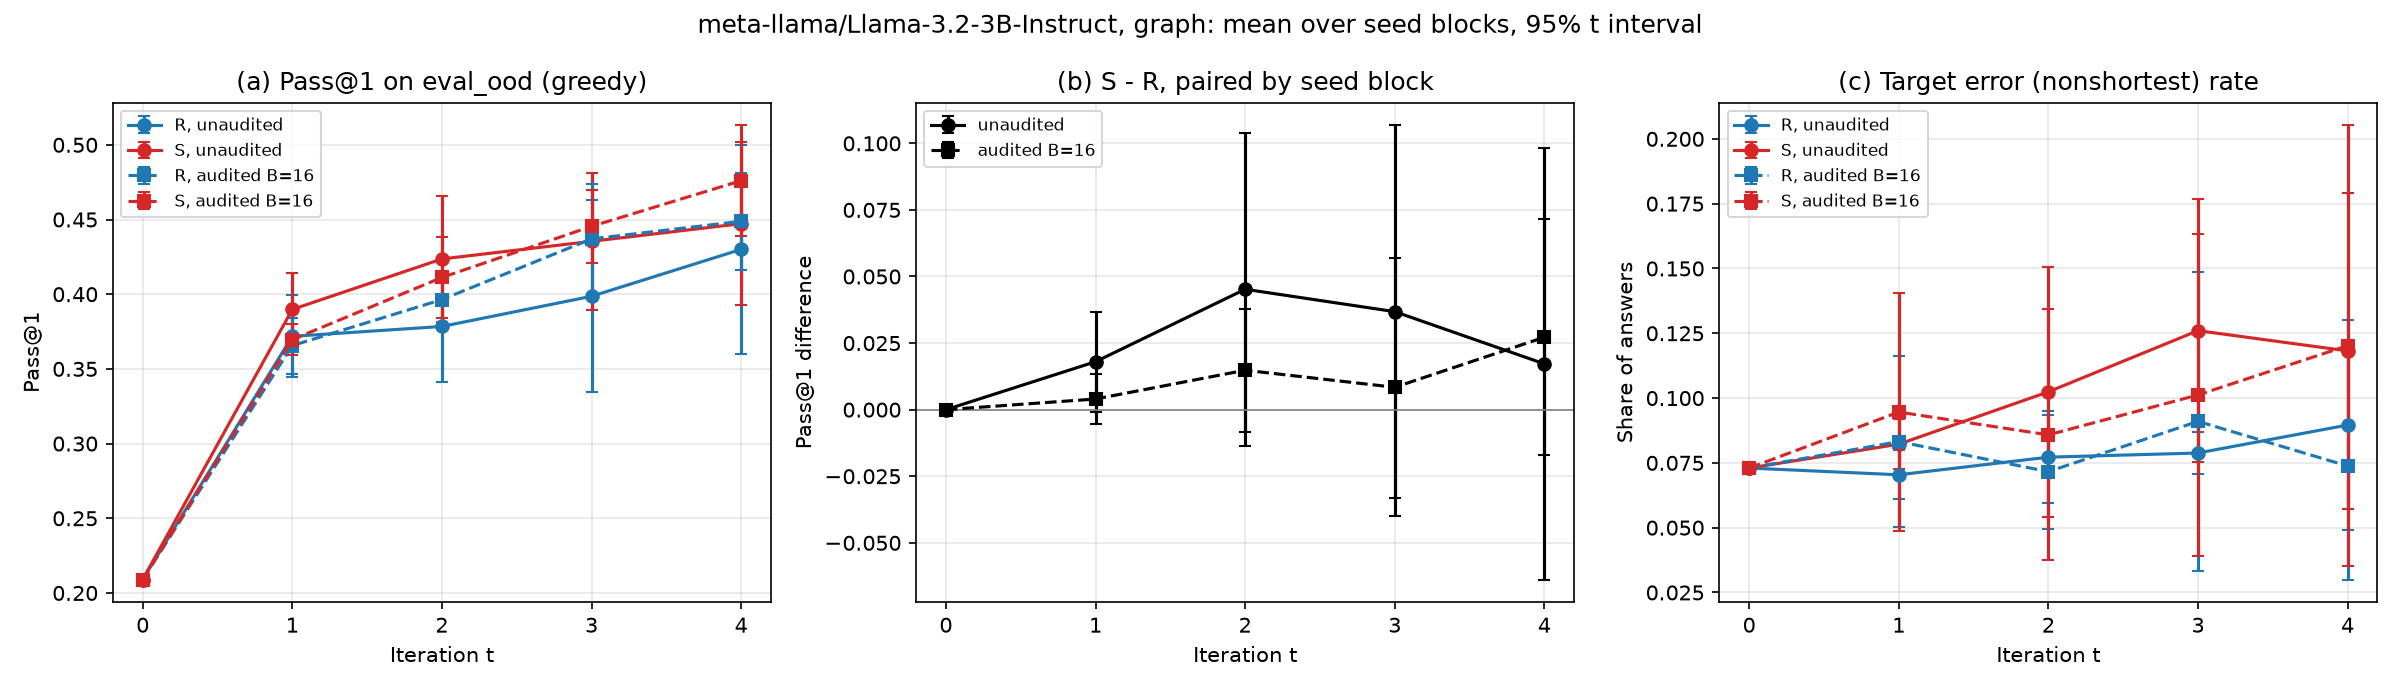
\includegraphics[width=0.90\linewidth]{figures/llama_four_round_raw/comparison_eval_ood_pass1.png}
\caption{Original joint comparison of unaudited and adaptive-audit
Llama-3.2-3B graph trajectories, ID (top) and OOD (bottom), for
rounds 0--4. Each middle panel reports paired $S-R$ accuracy
within each policy, not audited-minus-unaudited effects.}
\label{fig:llama-raw-comparison}
\label{fig:h100-id}
\label{fig:h100-ood}
\end{figure}

Auditing improves same-arm endpoint accuracy in mean
(Table~\ref{tab:audit-results}). Audited
OOD $S$ nonshortest incidence is $0.120$, versus $0.118$ without
auditing, so target-error suppression is not uniform.

\begin{figure}[H]
\centering
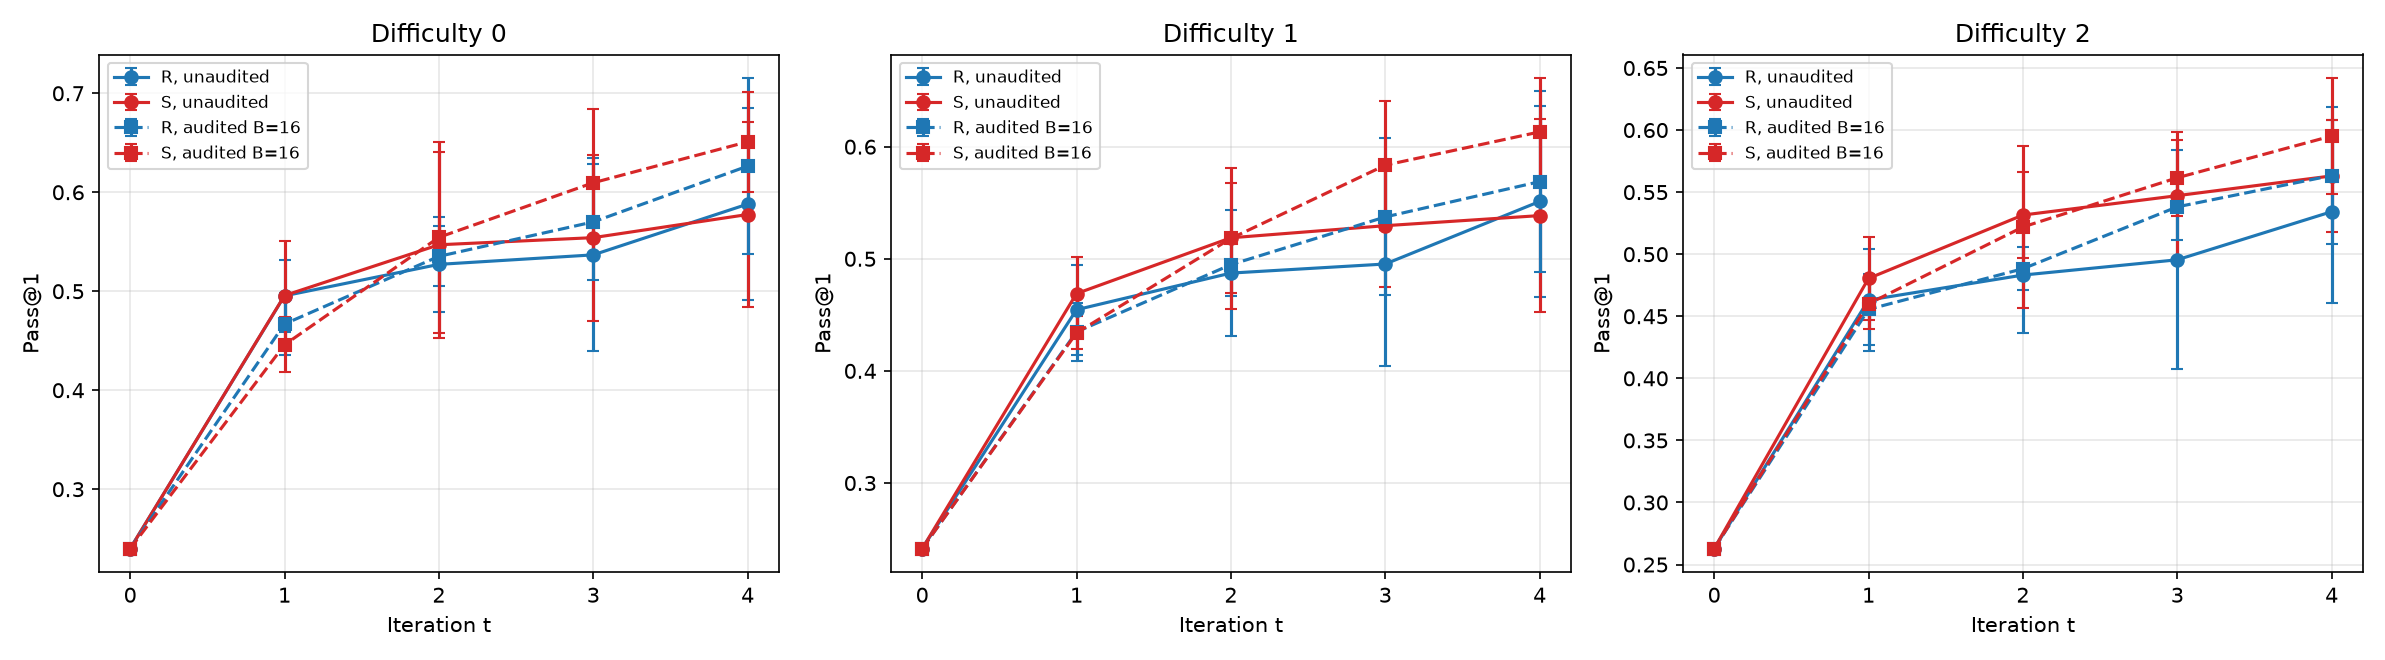
\includegraphics[width=0.90\linewidth]{figures/llama_four_round_raw/comparison_eval_id_by_difficulty.png}
\par\smallskip
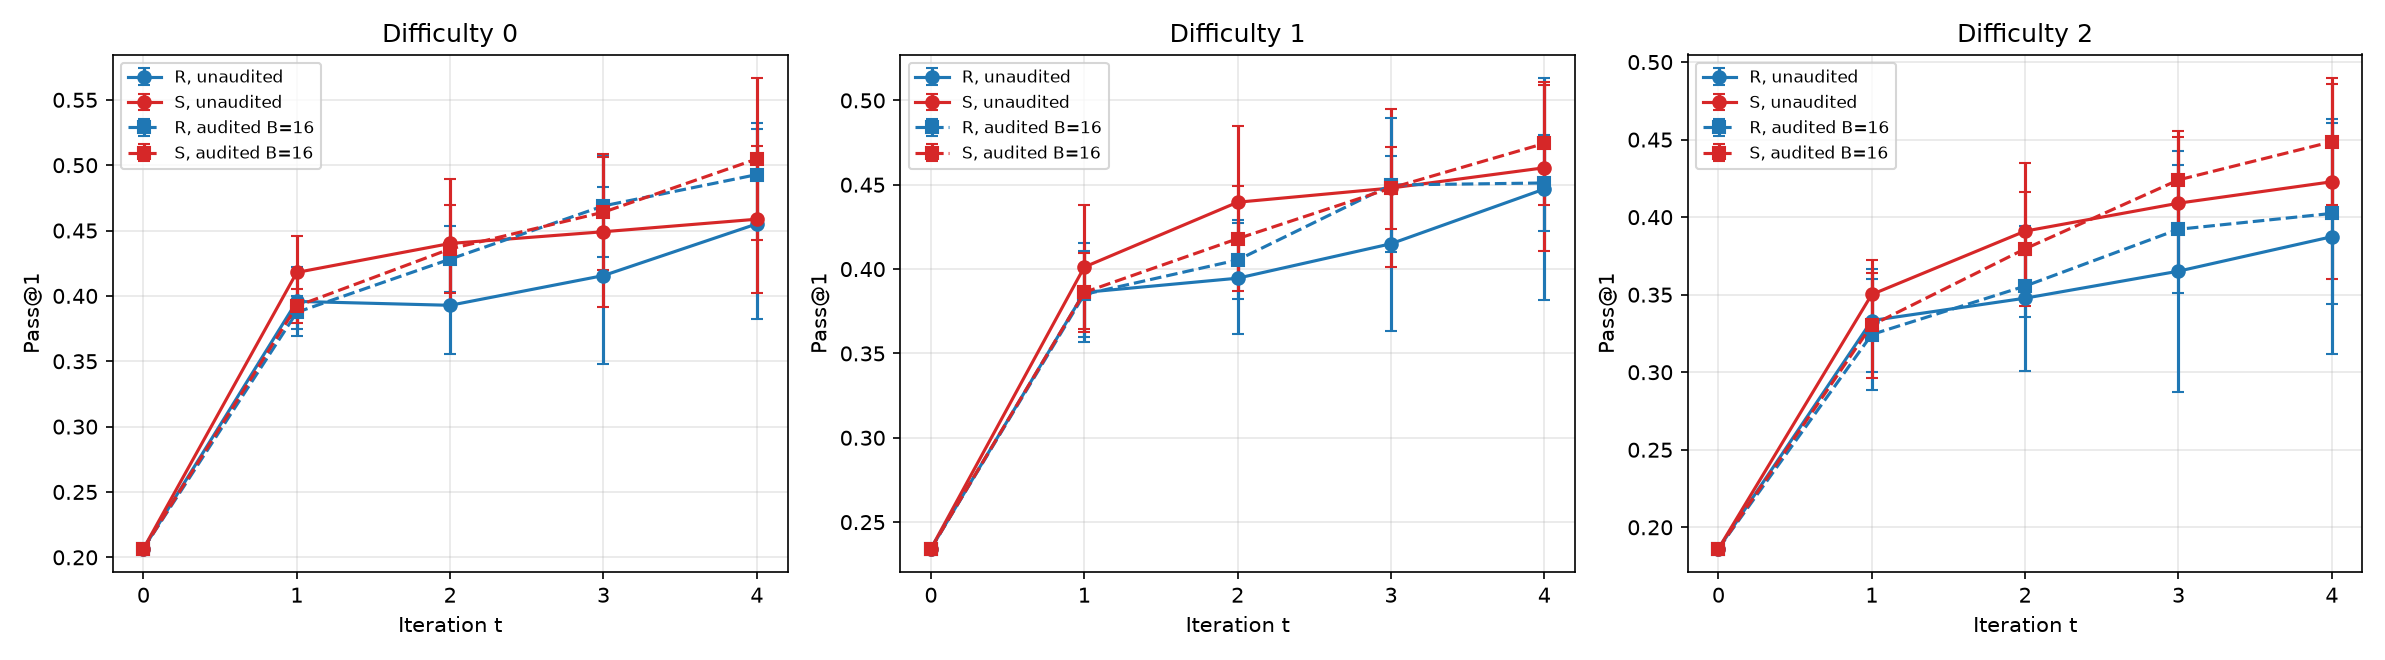
\includegraphics[width=0.90\linewidth]{figures/llama_four_round_raw/comparison_eval_ood_by_difficulty.png}
\caption{Original joint Llama-3.2-3B graph accuracy curves by
generator stratum, ID (top) and OOD (bottom), for rounds 0--4.
Both policies and both arms use the same question stratum at
each checkpoint. Counts and interval conventions follow
Figure~\ref{fig:llama-raw-unaudited-difficulty}.}
\label{fig:llama-raw-comparison-difficulty}
\label{fig:h100-difficulty}
\end{figure}

Both policies and both arms share the same question stratum at each
checkpoint. Separate vertical scales are retained, and the intervals
are not adjusted for comparisons across strata, rounds, or policies.
The joint curves complement the aggregate audit comparison without
providing an additional multiplicity-adjusted test.
\endgroup
